В процессе разработки программ программист неизбежно допускает ошибки. Для их обнаружения и исправления существует немало подходов: написание автоматических тестов, ручное тестирование, сохранение некоторой информации в лог, отладка и многие другие. Как правило, используется сразу несколько. В данной работе нас будет интересовать поиск ошибок при помощи отладчика.

\begin{definition}\label{debugger:definition}
	Отладчик --  компьютерная программа, предназначенная для поиска ошибок в других программах, ядрах операционных систем, SQL-запросах и других видах кода. Отладчик позволяет выполнять трассировку, отслеживать, устанавливать или изменять значения переменных в процессе выполнения кода, устанавливать и удалять контрольные точки или условия остановки и т.д.\cite{wiki:debugger}
\end{definition}

\noindent Отладчик позволяет увидеть состояние исполняемой программы:

\begin{itemize}
	\item Текущая инструкция
	\item Стек вызовов
	\item Значение локальных переменных
	\item Состояние памяти
	\item Потоки (состояние и стеки)
\end{itemize}

\noindent И выполнить действия

\begin{itemize}
	\item Добавление точки останова
	\item Переход к следующей инструкции/внутрь функции/месту вызова текущей функции
	\item Установка указателя на текущую инструкцию (IP)
	\item Модификация значений в памяти
	\item Вычисление выражений
	\item и другие
\end{itemize}

\subsection{Отладка Java}

Java исполняется на виртуальной машине JVM, поэтому средства для отладки предоставляет 
JVM.

Вместе с JDK (Java Development Kit) поставляется отладчик - jdb \cite{debug:jdb}. Это очень простой отладчик с интерфейсом командной строки, его цель -- демонстрация части возможностей платформы Java по отладке программ (JPDA - Java Platform Debugger Architecture). 

Платформа предоставляет инструменты для отладки, которые могут быть использованы в отладчиках сред разработки.

\subsubsection{Архитектура JPDA}\label{jdpa}
Упрощенно, схема работы JPDA выглядит следующим образом

\vspace{1em}
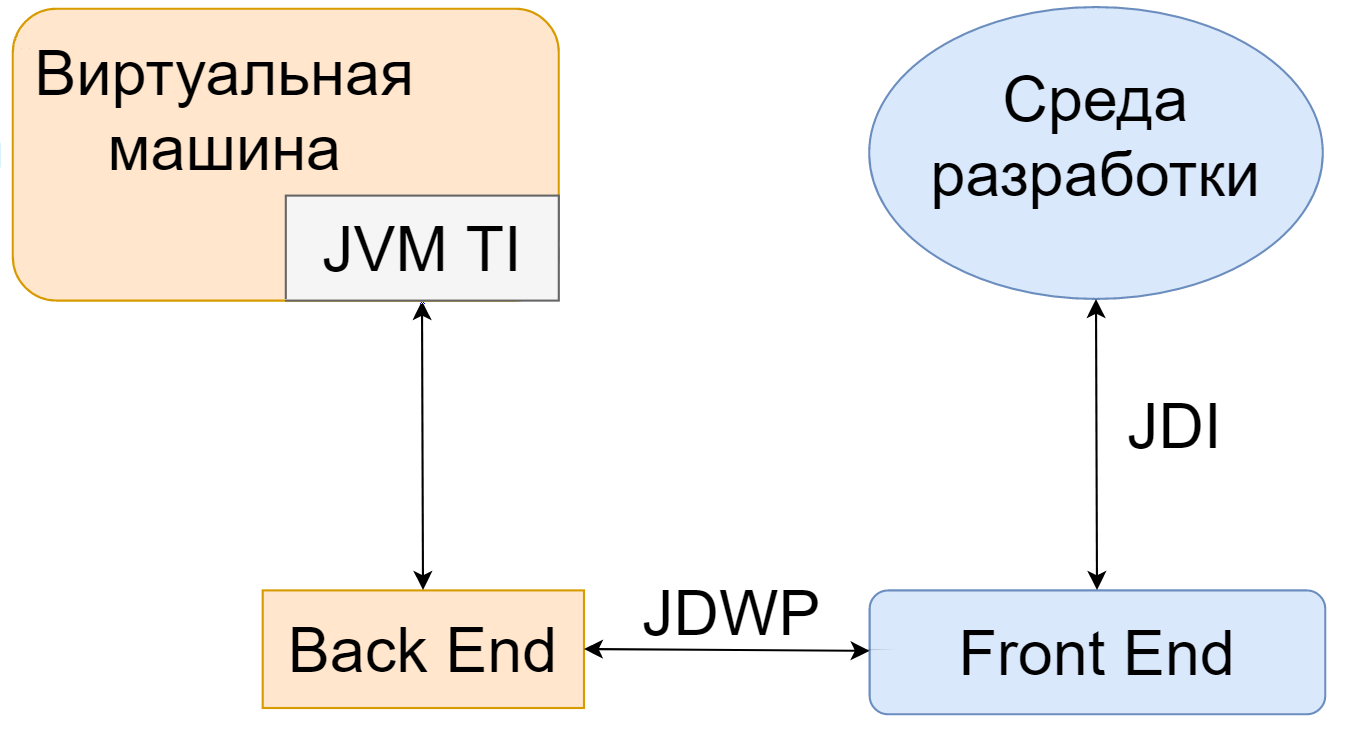
\includegraphics[scale=0.4]{chapter1/img/jdpa.png}

В блоках "Front End" и "Back End" скрыты детали реализации по обмену сообщениями -- очереди сообщений и потоки, обрабатывающие эти сообщения.

JPDA состоит из трех частей:
\begin{itemize}
	\item JVM TI -- Java VM Tool Interface - описывает сервисы, которая предоставляет виртуальная машина для отладки. 
	\item JDWP -- Java Debug Wire Protocol - протокол общения между отладчиком и виртуальной машиной. Описывает формат сообщений между отладчиком и JVM, создавая дополнительную абстракцию и позволяя использовать технологии для написания отладчиков.
	\item JDI -- Java Debug Interface - высокоуровневый Java интерфейс для взаимодействия с виртуальной машиной. Поставляется вместе с JDK, входит в пакет сom.sun.jdi. Позволяет получить доступ к состоянию программы, а так же контролировать ход её исполнения. Содержит набор классов-посредников для сущностей отлаживаемой виртуальной машины (потоки, объекты, классы и т.д.). Эти классы позволяют вызывать методы, получать и модифицировать значения полей, получать уведомления о событиях, приостанавливать и возобновлять потоки исполнения.
\end{itemize}



